\chapter{Introduction}
\label{chap:introduction}
Consider robots in environements with movable obstacles. For robots it remains a hard problem to navigate and act in new, unseen environments. Most approaches controlling the robot and acting as the robot brain fall in one of two categories. The bulk falls into hierarchical approaches~\cite{kaelbling_hierarchical_2011,scholz_navigation_2016,krontiris_dealing_2015}, an hierarchical structure generally consists of an high-level and low-level component. The high-level task planner tries to understand and model the environment, suck gained knowledge is used to generate action sequences toward a desired goal. The high-level planner sends actions to a low-level module, that takes care of sending input signals toward the robot actuators. The high-level planner has a prediction horizon consisting of an action sequence, a long prediction horizon compared to the low-level planner which prediction horizon is maximal one action. Hierarchical structures genarally provide solutions which are computationally effecient but are hierarchical solutions, meaning the solutions found are are teh best feasible solutions in the task hierarchy they search. The quality of the solution depends on the hierarchy which are typically hand-coded and domain specific~\cite{vega-brown_asymptotically_2020}. Altanively to hierarchical approaches, solutions can be provided by searching in a joint configuration space of the robot and obstacles, where the robots configuration space is augmented with environment obstacles configuration spaces whilst also including dynamic constraints~\cite{hauser_multimodal_2010,berenson_manipulation_2009,jaillet_path_2013}. Such a joint configuration space suffers from a combinational explosion and is practically impossible to search. Finding an action sequence from searching in a joint configuration is exaustive, instead for example a search close to the the current configuration, let the robot track this incomplete solution toward a desired goal and search the joint configuration space again close to the new current configuration. different techniques exist to prevent searching in the entire joint configuration space.\bs

Robots in new unforeseen environments is a broad topic, let's narrow down the scope. Consider a simple robot without grippers or arms attached. By sending input toward the wheels the robot can drive around. The environment consists of a flat ground plane, the robot and movable obstacles which the robot can manipulate by pushing. This creates two different modes of dynamics (driving, pushing) different differential constraints apply to the different modes, the different modes of dynamics result in a piecewise-analytic configuration space which hardens motion planning considerably~\cite{vega-brown_asymptotically_2020}. Whilst the robot can interact with the obstacles in the environment, there is no prior information provided to the robot (e.g. weight, friction coefficient) other than the shape and pose of the obstacle. By interaction with obstacles the robot can generate a system model, describing the expected trajactory of an obstacle as result of a push from the robot. The robot is tasked to relocate a subset of obstacles by means of pushing obstacles. \bs

Applicable to such an robot environment three topics in robotics investigated, these topics are \textbf{motion planning}, \textbf{placing obstacles at target locations}, and \textbf{learning obstacle dynamics}. Whilst individually a considerable amount of research is done in these topics (motion planning~\cite{lavalle_planning_2006,elbanhawi_samplingbased_2014,kingston_samplingbased_2018,chen_fast_2018}, pusing obstacles to target locations~\cite{arruda_uncertainty_2017,mericli_pushmanipulation_2015,toussaint_sequenceofconstraints_2022,stuber_let_2020,stuber_featurebased_2018,bauza_dataefficient_2018}, learning obstacle dynamics~\cite{seegmiller_vehicle_2013,cong_selfadapting_2020}), combining 2 out of these 3 topics is lesser researched and combining all three even scarcer.\bs

\citeauthor{vega-brown_asymptotically_2020} investigated motion planning in a piecewise-analytic configuration space to relocate obstacles~\cite{vega-brown_asymptotically_2020}. Whilst an an optimal plan is obtained with probability one with infinite samples, the algorithm does not learn the pushing relation between the robot and the obstacles. The ability to learn push dynamics greatly broadens the variety of obstacles a robot can push. Realisticly robots in warehouses, hospitals or supermarkets might encounter a variety of different obstacles, but learning dynamics inavitably leads to system model mismatch. An motion planning algorithm should be competable with learned system models and take model mismatch into account.\bs

\citeauthor{wang_affordancebased_2020} takes pushing objects to target location out of the equation and only focussus on the \ac{NAMO} problem. Learning interaction by embedding unknown obstacles with affordance information followed by planning with a contact-implicit motion planner toward a robot goal location~\cite{wang_affordancebased_2020}. By removing pushing obstacles the problem simplifies, the piecewise-analytic configuration spaces simplifies to a configuration space.\bs

\citeauthor{vega-brown_asymptotically_2020} and \citeauthor{wang_affordancebased_2020} both combine 2 of the 3 topics allowing for an more in depth analysis but avoiding the problems introduced by combining all 3 topics. \citeauthor{sabbaghnovin_model_2021} combines all three topics: motion planning, placing obstacles at target location and learning obstacle dynamics. He proposes to obtain system models by analysing and converting a limited set of robot-obstacle test pushes using Bayesion regression to predict model parameters. Path planning is the result of solving an proposed mixed-integer convex optimization~\cite{sabbaghnovin_optimal_2016} which is tracked by \ac{MPC} control.\bs

As will be seen in upcoming sections, this thesis proposes a method which combining the 3 topics relying on a technique known as \textbf{backward induction}, \textbf{backward tracing} or \textbf{backward search}. The proposed method in this thesis and \citeauthor{sabbaghnovin_model_2021} proposed method solve comparible types of problems using vastly different techniques, allowing for easy comparinson between the the results of \citeauthor{sabbaghnovin_optimal_2016} and the results from the proposed method in this thesis.\bs

\section{Problem Description}
Tests are performed in a robot simulation environment, let's start with defining the environment.\\Let tuple $\left\langle \text{Origin}, \text{Ground Plane}, \text{Obstacles}, E \right\rangle$ fully define a robot environment where:\bs

\par\smallskip\noindent
\centerline{\begin{minipage}{0.8\textwidth}
\begin{enumerate}

  \item[Origin] Static point in the environment with a $x$-, $y$- and $z$-axis. Any point in the environment has a linear and an angular position and velocity with respect to the origin \vspace{0.5\baselineskip}
 \item[Ground Plane] A flat plane parallel with the Origin's $x$- and $y$- axis. Obstacles cannot pass through the ground plane and meet sliding friction when sliding over the ground plane. \vspace{0.5\baselineskip}
 \item[Obstacles] A 3-dimensional body with shape and uniformly destributed mass. An obstacle has a state consisting of the linear and angular position and velocity are between the obstacles center of mass and the origin. Examples of obstacles are given in \cref{fig:example_obstacles}. \vspace{0.5\baselineskip}
  \item[$E$] A set of motion equation describing the behaviour of obstacles such as gravity, interacteraction with the ground plane or interaction with other obstacles. The motion equations coinside with the true dynamics. \vspace{0.5\baselineskip}
\end{enumerate}
\end{minipage}}
\par\smallskip


enva flat ground plane, gravity, 3-dimensional obstacles the bbb with gravity pulling every obstacle and the robot perpendicular toward the ground plane.


\subsection{Task}
\todo[inline]{describe the piecewise analitic configuration space, joint configuration space introduce NP-space hard problem}

\subsection{Assumptions}
\label{subsec:assumptions}
% what do you want to tell? -> assumptions are here too ease the 
In order to simplify the problem described in the problem description, a number of assumptions are taken, which are now listed. 

\begin{assumption}
\label{assumption:closed_world}
\textbf{Closed-World Assumption:} Objects are manipulated, directly or indirectly only by the robot. Objects cannot be manipulated by influences from outside the environment.
\end{assumption}

\begin{assumption}
\label{assumption:quasi_static}
\textbf{Quasi-Static Assumption:} Velocities are small enough that inertial forces are negligible~\cite{stuber_let_2020}.
\end{assumption}

\begin{assumption}
\label{assumption:perfect_obstacle_sensor}
\textbf{Perfect Obstacle Sensor Assumption:} the robot has full access to the poses and geometry of all obstacles in the environment at all times.
\end{assumption}

\begin{assumption}
\label{assumption:order_does_not_matter}
\textbf{Tasks are Commutative} Tasks exist of multiple obstacles with specified target positions. The order in which obstacles are pushed toward their target position is commutative.
\end{assumption}

\begin{assumption}
\label{assumption:no_tipping}
\textbf{Obstacles do not tip over} Movable obstacles slide if pushed.
\end{assumption}
\todo[inline]{should I put assumption in task are comm and not tip over? or remove the other "Assumption" for consistnecy?}


The assumptions taken serve to simplify the problem of task completion. Note that in \cref{sec:future_work} insight is given to remove all but Assumption 2. By removing assumptions completing tasks becomes a harder problem, but a more realistic problem closer to the real world applications.\bs

Assumptions might have certain implications, which are now listed. The \hyperref[assumption:closed_world]{closed-world assumption} implies that obstacles untouched by the robot and with zero velocity component remain at the same position. Completed subtasks are therefore assumed to be completed for all times after completion time.\\The \hyperref[assumption:quasi_static]{quasi-static assumption} allows to neglect complex dynamics, which in many cases are negligible. To ensure that complex dynamics do not become significant during testing, a maximum robot speed or accelaration is enforced.\\The \hyperref[assumption:perfect_obstacle_sensor]{perfect obstacle sensor assumption} simplifies a sensor setup, it prevents Lidar-, camera setups and for tracking setups with aruco or other motion caputer markers. The existence of a single perferct measurement wipes away the need to combine measurements from multiple sources with sensor fusion algorithms, such as Kalman filtering \cite{verhaegen_filtering_2007}.\\Certain tasks are only feasible if performed in a certain order (e.g. the Tower of Hanoi), the \hyperref[assumption:order_does_not_matter]{tasks are commutative assumption} allows to focus only on a single subtask since it does not affect the completion or feasibility of other subtasks.\\The \hyperref[assumption:no_tipping]{Obstacles do not tip over} ensures that obstacles do not tip over and suddenly have vastly different dynamical properties. In practice obstacles will not be higher than the minimum width of the obstacle, and spheres are excluded since rolling essentially is tipping. 
\todo[inline]{should I put these implications right below the assumption itself?}

\subsection{The Simulation Environment}
Testing in a simulation environment has been done using the URDF Gym Environment~\cite{spahn_urdfenvironment_2022}, a 100\% python environment build upon the PyBullet library \cite{coumans_pybullet_2016}. The code created during the thesis can be found on \href{https://gitlab.tudelft.nl/airlab-delft/msc_projects/msc_gijs_groote}{GitLab} and \href{https://github.com/GijsGroote/semantic-thinking-robot}{GitHub}. Experiments ran on standart TU Delft laptop: HP ZBook Studio x360 G5,running OS: Ubuntu 22.04.1 LTS x86\_64, CPU: Intel i7-8750H (12) @ 4.100GHz, GPU: NVIDIA Quadro P1000 Mobile.\bs

The simulation environment provides many different robot, 2 simple robots are selected to perform tests, they are displayed in \cref{fig:example_robots}, various obstacles are displayed in \cref{fig:example_obstacles}.

\begin{figure}[H]
    \centering
    \begin{subfigure}{.5\textwidth}
    \centering
    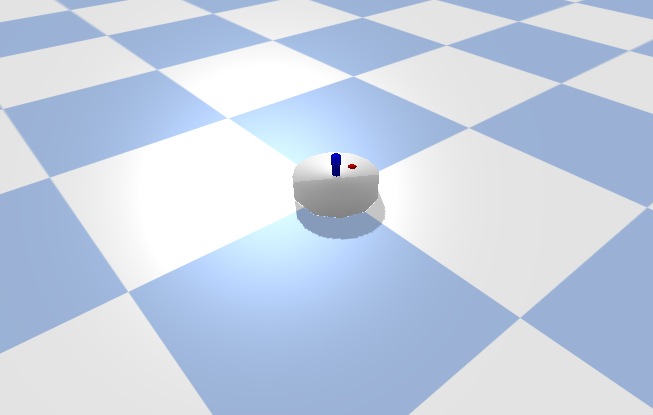
\includegraphics[width=0.8\textwidth]{figures/point_robot.png}
    \caption{The holonomic point robot\\the 2 inputs drive the robot in $x$ and in $y$ direction}
    \label{subfig:example_point_robot}
    \end{subfigure}%
    \begin{subfigure}{.5\textwidth}
    \centering
    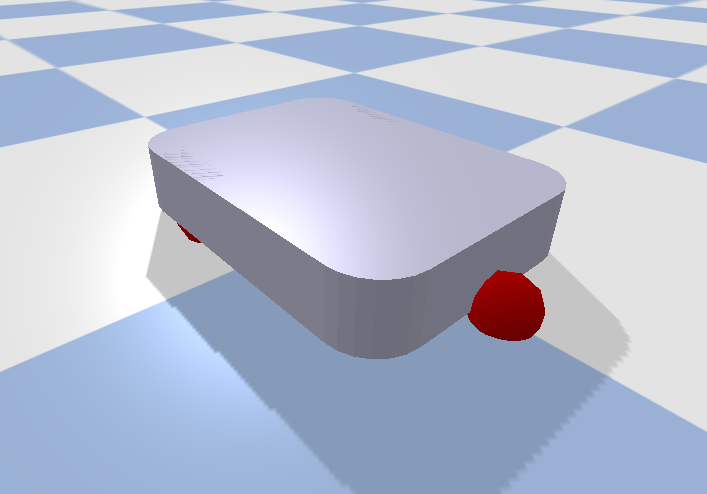
\includegraphics[width=0.8\textwidth]{figures/boxer_robot.png}
    \caption{The nonholonomic boxer robot\\the first input drives the robot forward/backward\\the second rotates the robot}
    \label{subfig:example_boxer_robot}
    \end{subfigure}%
    \caption{Robots used for testing, for either robot an velocity and a accelaration input exists, in total 4 different robots are used}
    \label{fig:example_robots}
\end{figure}
\todo[inline]{zoom in a bit on these 2 cute robots}

\begin{figure}[H]
    \centering
    \begin{subfigure}{.5\textwidth}
    \centering
    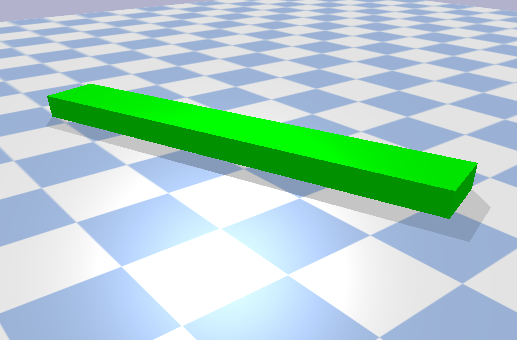
\includegraphics[width=0.8\textwidth]{figures/box_obstacle.png}
    \caption{A box obstacle}
    \end{subfigure}%
    \begin{subfigure}{.5\textwidth}
    \centering
    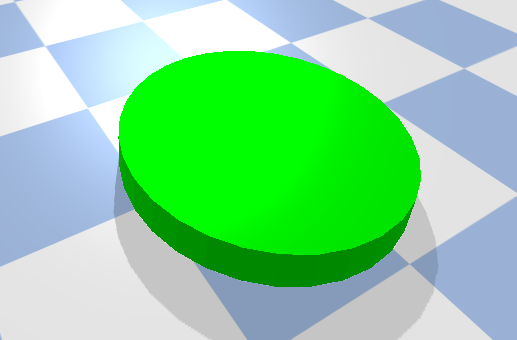
\includegraphics[width=0.8\textwidth]{figures/cylinder_obstacle.png}
    \caption{A cylinder obstacle}
    \end{subfigure}%
    \caption{Various obstacles in the robot environment}
    \label{fig:example_obstacles}
\end{figure}



\section{Research Question}

\textbf{Main research question:}
\begin{center}
\label{researchquestion:main}
\large
How do obstacles' system models learned by a nonprehensile manipulation robot during\\  task execution improve global task planning?
\end{center} 

\textbf{Research subquestion:}
\begin{enumerate}
    \item\label{researchsubquestion:does_it_work} How does backtracing~\cite{krontiris_dealing_2015} while remembering interactions with unknown obstacles compare to not remembering learning interactions over time?
    \item\label{researchsubquestion:does_it_compare} Can the proposed method combine learning and planning for push en drive applications? Can the proposed method complete tasks, and how does it compare against the state of the art? 
\end{enumerate}


\section{Report Structure}


\todo[inline]{Create the report structure when the report structure does not change any more}
